\chapter{OpenCV}\label{c:opencv}

OpenCV (Open Source Computer Vision Library) is a library of thousands
of algorithms for various applications in computer vision and machine
learning. It has C++, C, Python, Java and MATLAB interfaces and supports
Windows, Linux, Android and Mac OS. In this tutorial, we will explain
basic features of this library, including the implementation of a simple
example.

\section{Overview}\label{overview}

OpenCV has countless functions for image and videos processing. The
pipeline starts with reading the images, low-level operations on pixel
values, preprocessing e.g.~denoising, and then multiple steps of
higher-level operations which vary depending on the application. OpenCV
covers the whole pipeline, especially providing a large set of library
functions for high-level operations. A simpler library for image
processing in Python is Scipy's multi-dimensional image processing
package (scipy.ndimage).

\section{Installation}\label{installation}

OpenCV for Python can be installeed on Linux in multiple ways, namely
PyPI(Python Package Index), Linux package manager (apt-get for Ubuntu),
Conda package manager, and also building from source. You are
recommended to use PyPI. Here's the command that you need to run:

\begin{verbatim}
pip install opencv-python
\end{verbatim}

This was tested on Ubuntu 16.04 with a fresh Python 3.6 virtual
environment. In order to test, import the module in Python command line:

\begin{verbatim}
>>> import cv2
\end{verbatim}

If it does not raise an error, it is installed correctly. Otherwise, try
to solve the error.

For installation on Windows, see:

  \url{https://docs.opencv.org/3.0-beta/doc/py_tutorials/py_setup/py_setup_in_windows/py_setup_in_windows.html#install-opencv-python-in-windows}

Note that building from source can take a long time and may not be
feasible for deploying to limited platforms such as Raspberry Pi.

\section{A Simple Example}\label{a-simple-example}

In this example, an image is loaded. A simple processing is performed,
and the result is written to a new image.

\subsection{Loading an image}\label{loading-an-image}

\begin{verbatim}
%matplotlib inline
import cv2

img = cv2.imread('opencv_files/4.2.01.tiff') 
\end{verbatim}

The image was downloaded from USC standard database:

  \URL{http://sipi.usc.edu/database/database.php?volume=misc&image=9}

\subsection{Displaying the image}\label{displaying-the-image}

The image is saved in a numpy array. Each pixel is represented with 3
values (R,G,B). This provides you with access to manipulate the image at
the level of single pixels. You can display the image using imshow
function as well as Matplotlib's imshow function.

You can display the image using imshow function:

\begin{verbatim}
cv2.imshow('Original',img)
cv2.waitKey(0)
cv2.destroyAllWindows()
\end{verbatim}

or you can use Matplotlib. If you have not installed Matplotlib before,
install it using:

\begin{verbatim}
pip install matplotlib
\end{verbatim}

Now you can use:

\begin{verbatim}
import matplotlib.pyplot as plt
plt.imshow(img)
\end{verbatim}

which resuts in 

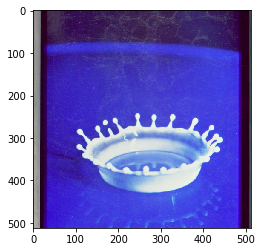
\includegraphics[width=0.15\textwidth]{opencv_files/output_5_1.png}


\subsection{Scaling and Rotation}\label{scaling-and-rotation}

Scaling (resizing) the image relative to different axis

\begin{verbatim}
res = cv2.resize(img,
                 None,
                 fx=1.2, 
                 fy=0.7, 
                 interpolation=cv2.INTER_CUBIC)
plt.imshow(res)
\end{verbatim}

which results in 

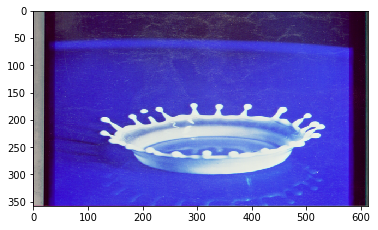
\includegraphics[width=0.15\textwidth]{opencv_files/output_7_1.png}


Rotation of the image for an angle of t

\begin{verbatim}
rows,cols,_ = img.shape
t = 45
M = cv2.getRotationMatrix2D((cols/2,rows/2),t,1)
dst = cv2.warpAffine(img,M,(cols,rows))

plt.imshow(dst)
\end{verbatim}

which results in 

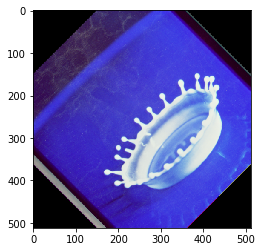
\includegraphics[width=0.15\textwidth]{opencv_files/output_9_1.png}

\subsection{Gray-scaling}\label{gray-scaling}

\begin{verbatim}
img2 = cv2.cvtColor(img, cv2.COLOR_BGR2GRAY)
plt.imshow(img2, cmap='gray')
\end{verbatim}

which results in 

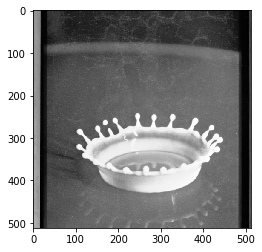
\includegraphics[width=0.15\textwidth]{opencv_files/output_11_1.png}


\subsection{Image Thresholding}\label{image-thresholding}

\begin{verbatim}
ret,thresh =    cv2.threshold(img2,127,255,cv2.THRESH_BINARY)
plt.subplot(1,2,1), plt.imshow(img2, cmap='gray')
plt.subplot(1,2,2), plt.imshow(thresh, cmap='gray')
\end{verbatim}

which results in 

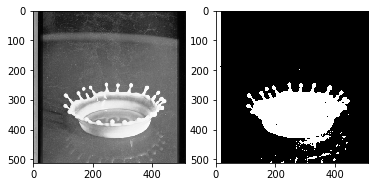
\includegraphics[width=0.3\textwidth]{opencv_files/output_13_1.png}


\subsection{Edge Detection}\label{edge-detection}

Edge detection using Canny edge detection algorithm

\begin{verbatim}
edges = cv2.Canny(img2,100,200)

plt.subplot(121),plt.imshow(img2,cmap = 'gray')
plt.subplot(122),plt.imshow(edges,cmap = 'gray')
\end{verbatim}

which results in 

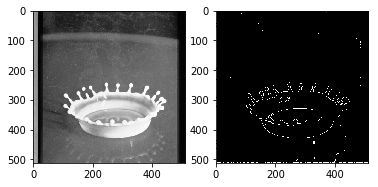
\includegraphics[width=0.3\textwidth]{opencv_files/output_15_1.png}


\section{Additional Features}

OpenCV has implementations of many machine learning techniques such as
KMeans and Support Vector Machines, that can be put into use with only
a few lines of code. It also has functions especially for video
analysis, feature detection, object recognition and many more. You can
find out more about them in their website

\URL{https://docs.opencv.org/3.0-beta/index.html}

OpenCV was initially developed for C++ and still has a focus on that
language, but it is still one of the most valuable image processing
libraries in Python.
